\documentclass{beamer}
\usepackage{natbib}
\usepackage{graphicx}
\hypersetup{colorlinks,linkcolor=blue,urlcolor=blue}

\title{Packages for Microbiome Data Vis}
\author{Kris Sankaran}

\begin{document}

\begin{frame}
  \frametitle{Motivation}

\begin{itemize}
\item When working with static visualizations, it's common to generate many
  versions of the same figure (``small multiples'')
  \begin{itemize}
  \item E.g., plotting time series for each species, genus, family, ...
  \item For some problems, this can become unmanageable
  \end{itemize}
\end{itemize}
\begin{figure}
  \centering
  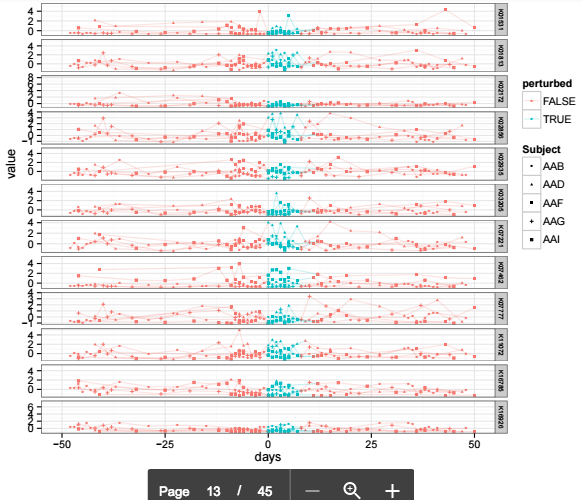
\includegraphics[width=0.6\textwidth]{many_series.png}
  \caption{45 pages of small multiples isn't very useful. \label{fig:many_series} }
\end{figure}
\end{frame}

\begin{frame}
  \frametitle{Visualization principles}

  \begin{itemize}
  \item Linking: Combine alternative views of the same data
  \item Focus plus context: Allow quick navigation between large (context) and
    small (focus) scales
  \end{itemize}
\begin{figure}
  \centering
  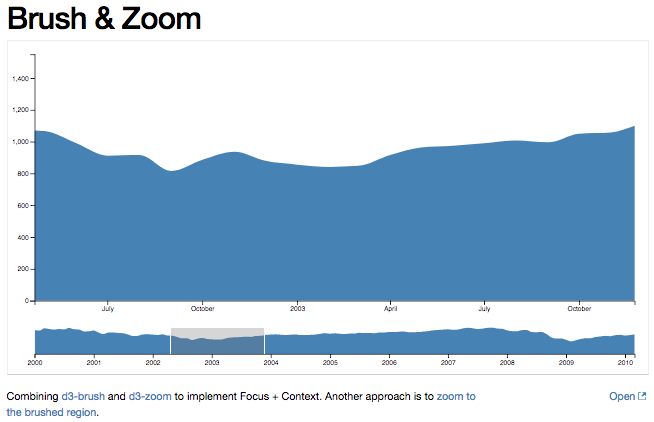
\includegraphics[width=0.6\textwidth]{d3-focus-context}
  \caption{The main panel is the focus, while the brushed series on the bottom
    provides context.}
\end{figure}

\end{frame}

\begin{frame}
  \frametitle{My packages}

\begin{itemize}
\item Multivariate analysis: \href{https://github.com/krisrs1128/mvarVis}{Package} and
  \href{http://statweb.stanford.edu/~kriss1/mvarVis\_d3\_examples.html}{examples}.
\item Collections of time series:
  \href{https://krisrs1128.github.io/treelapse/}{treelapse} (examples within)
\item Cluster centroids: \href{http://statweb.stanford.edu/~kriss1/hclust.html}{Example}
  and \href{https://github.com/krisrs1128/centroidview}{draft package}
\end{itemize}
\begin{figure}
  \centering
  \includegraphics[width=0.9\textwidth]{my-packages}
\end{figure}


\end{frame}
\begin{frame}
  \frametitle{Interactivity in R}

\begin{itemize}
\item \href{https://shiny.rstudio.com/gallery/}{Shiny}: Web interfaces that to R
  scripts. See also
  \href{http://joey711.github.io/shiny-phyloseq/}{Shiny phyloseq}.
\item \href{https://plot.ly/r/}{plotly}: Interactive versions of common plot types.
\item \href{http://deltarho.org/docs-trelliscope/}{trelliscope}: Navigation
  across similar panels based on ``cognostics'' (summary statistics).
\item \href{http://gallery.htmlwidgets.org/}{htmlwidgets}: R interfaces to
  javascript visualizations.
\end{itemize}
\begin{figure}
  \centering
  \includegraphics[width=0.9\textwidth]{interactivity-R}
\end{figure}

\end{frame}

\end{document}
